\section{System Development}\label{sec:development}
\phantomsection

\subsection{Implementation}
\subsubsection{Scientific environment}
With a theoretical background and a system design, it is possible to present the implementation phase of the project. Roughly the system is decoupled into 2 independent parts. The first one represents the training of the system and the resulting model. The second one is the end-user application. Even though the two parts are independent from each other, they actually reuse the Digital Signal Processing module. Clearly both modules deal with processing raw WAV data.

The project with the codename ``Nosnore'' is written entirely in Python programming language, CPython interpreter version $2.7$. The main arguments to use Python as the main and only programming language are the following:

\begin{itemize}[topsep=5pt, partopsep=0pt,itemsep=3pt,parsep=1pt]
 \item since the project is released under open source MIT license, it is an advantage that Python itself is an open source project;
 \item nevertheless readability of a programming language is a disputable fact, generally Python syntax is considered well thought out, easy to read and maintain;
 \item Python is a very popular language between regular developers and researches, which diminished the gap of contributing to the project or reusing some of its functionality;
 \item it represents the perfect balance between a high and low level programming language, unlike many other languages like R, Julia or even Matlab/Octave although the scientific environments;
 \item acting as a wrapper to many Matlab and C subroutines that can be called from Python;
 \item developed standardized documentation system, which makes sharing and collaboration even easier;
 \item large variety of free libraries for scientific computations, like NumPy, SciPy, Matplotlib, Sklearn, etc;
 \item hierarchical module system;
 \item the standard library is mostly cross-platform code;
 \item Kivy is a cross-platform framework, which makes is possible to deploy Python application on Windows, OS X, Linux, Android and iOS.
\end{itemize}

As a conclusion Python is a complete programming solution and it was used both for scientific computations and for the high level application. Moreover since everything is build around Python, it is easy to transfer the functionality to a web server or any other extra system architecture layer.

For the development of this project a special scientific environment was used, called Anaconda, \cite{anaconda}. Anaconda offers more than 195 most popular Python packages for science, math, engineering, data analysis. It is available on multiple platforms and contains the latest package updates. Anaconda is build using Python virtual environment, hence doesn't affect the global installation or the global packages. It also provides an interface and a package manager for manipulating the scientific environment.

A vital packages for scientific computation in Python represents Numpy, \cite{numpy}. It offers powerful N-dimensional array object manipulations, a set of sophisticated functions, tools for integrating C/C++, Fortran functions, linear algebra, Fourier transforms and has many other capabilities. Numpy is considered the building block of all other Python scientific packages.

Scipy (\cite{scipy}) is a Python-based ecosystem of open-source software for mathematics, science, and engineering. It includes such packages as Numpy, Pandas for data structures and analysis, Matplotlib for 2D plotting, Sympy for symbolic computations, iPython enhanced interactive console. SciPy also represents not only a stack of scientific packages, but also a library to provide user-friendly and efficient numerical routines such as routines for numerical integration and optimization.

Specifically for machine learning there exists a package called Scikit-learn, \cite{scikit-learn}. It is based on Numpy, Scipy and Matplotlib and maintains simple and efficient tools for data mining and data analysis. It contains algorithms for supervised, unsupervised, semi-supervised machine learning algorithms, which can perform preprocessing regression, classification, clustering, etc. 

All the packages have comprehensive and extensive documentation with good examples and a big community to develop the scientific ecosystem in Python. Therefore it is easy to use them.

\subsubsection{Signal processing of snore waves}

The DSP module is build using scientific packages with necessary adaptations described above. Since it DSP doesn't involve a hierarchy or classification of objects, it uses the procedural paradigm to construct algorithms. Nevertheless there is signal class presented in \ref{list1}, which encapsulated and performs basic functionality. All the other procedures are stored in functions in a common module.

All the important computations are performed by a worker, which calls the DSP functions to perform the processing and get the features from the PSD. In \ref{list2} it takes each signal, splits it into smaller signals and applies the filtering, normalization and other methods. Eventually the valuable information represents the features, which are obviously named as ``features'' in the code.

\lstinputlisting[language=Python, caption={Worker Python code}, label=list2]{../sourcecode/worker.py}

Low pass filtering is achieved using Butterworth filter presented in \ref{list11}. Butterworth filters (lowpass, bandpass, highpass, and bandstop digital and analog filters) are characterized by a magnitude response that is maximally flat in the passband and monotonic overall. Butterworth filters sacrifice rolloff steepness for monotonicity in the pass and stopbands. Unless the smoothness of the Butterworth filter is needed, an elliptic or Chebyshev filter can generally provide steeper rolloff characteristics with a lower filter order.

\lstinputlisting[language=Python, caption={Lowpass filter implementation}, label=list11]{../sourcecode/lowpass.py}

Normalization is done exactly as described in the domain analysis chapter, i.e. by using the standard deviation.

\lstinputlisting[language=Python, caption={Normalization function}, label=list12]{../sourcecode/normalize.py}

Even though the autocorrelation can be done using the relation \eqref{eq:accor}, it requires more computational power and hence more time. Therefore for autocorrelation it is reasonable to do the inverse FFT to the product of the real FFT and the conjugate of the real FFT as presented in \ref{list3}.

\lstinputlisting[language=Python, caption={Autocorrelation function code}, label=list3]{../sourcecode/autocorrelation.py}

In figure \ref{fig:snorewave} is presented the snore wave in raw form as it is received from the input device. By following all the DSP steps described in \ref{subsubsec:dsp} the signal will result into a set of formants relevant for the study displayed in \ref{fig:snorepsd}. From this point, it can be seen that PSD holds some important information about the signal, particularly the peaks. The biggest spike happens around $150$ unit of frequency. Along with that some of the peaks are as well quite persistent for all the sample data -- close to $50$, $70$, $100$, $200$ and the neighborhood of $300$. 

\begin{figure}[!ht]
\centering
  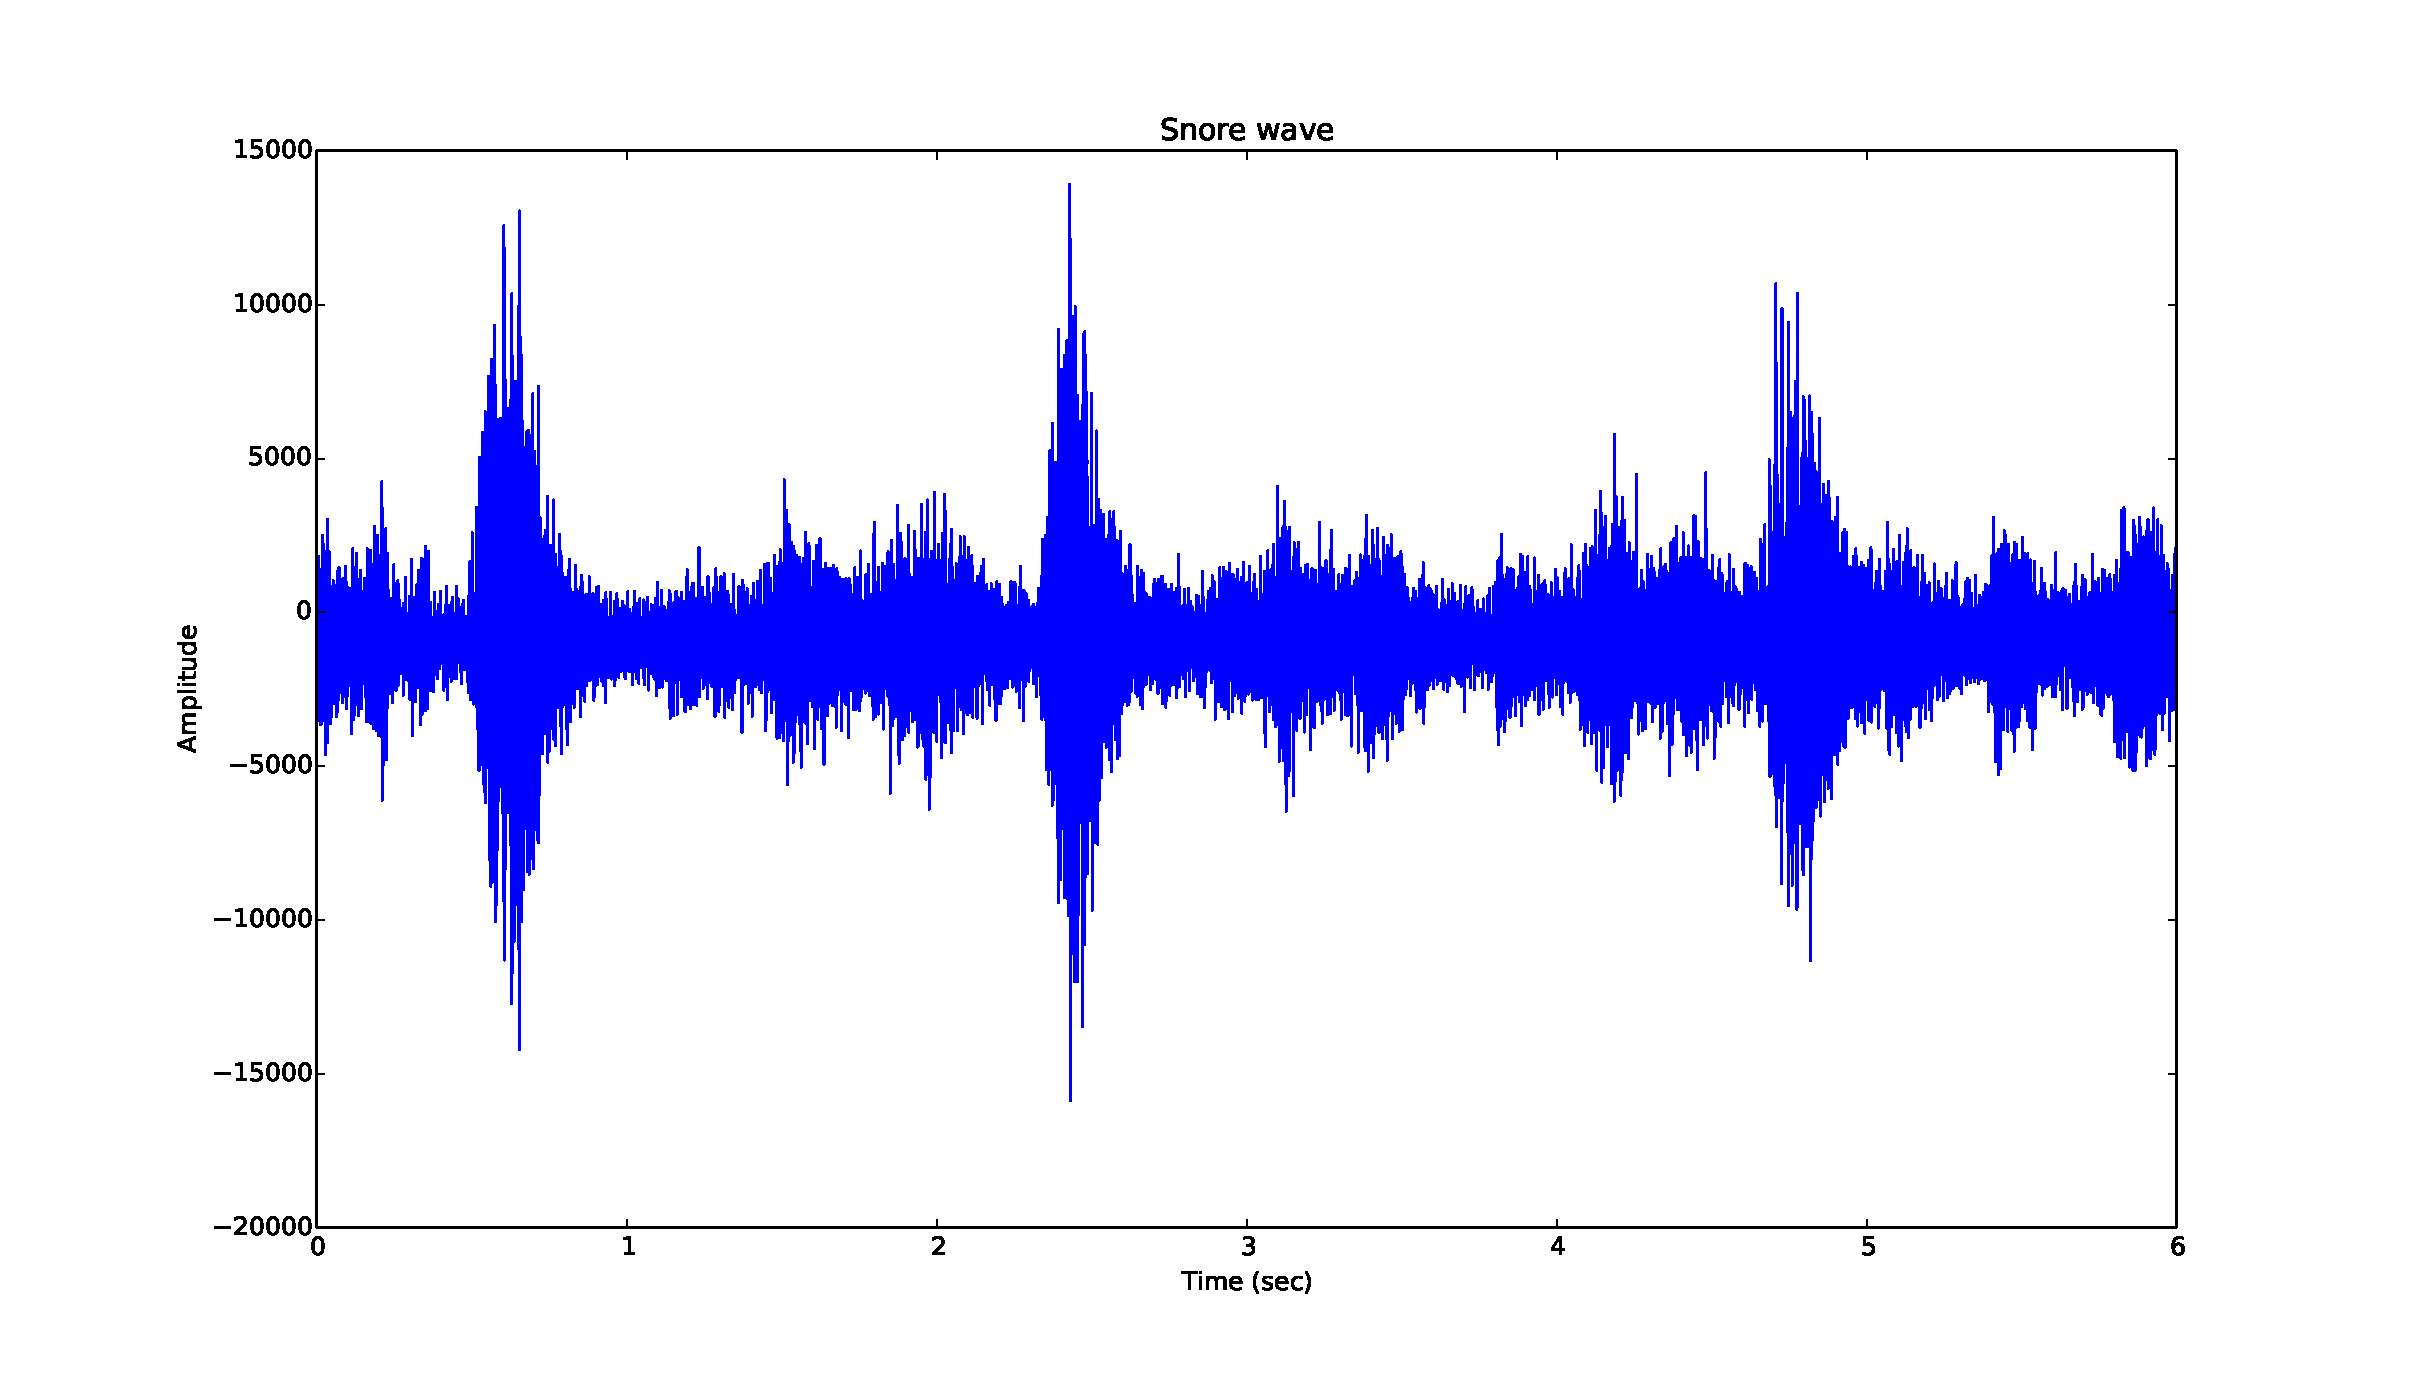
\includegraphics[width=15cm]{12_snorewave.eps}
\caption{Snore signal wave in time domain}
\label{fig:snorewave}
\end{figure}

\begin{figure}[!ht]
\centering
  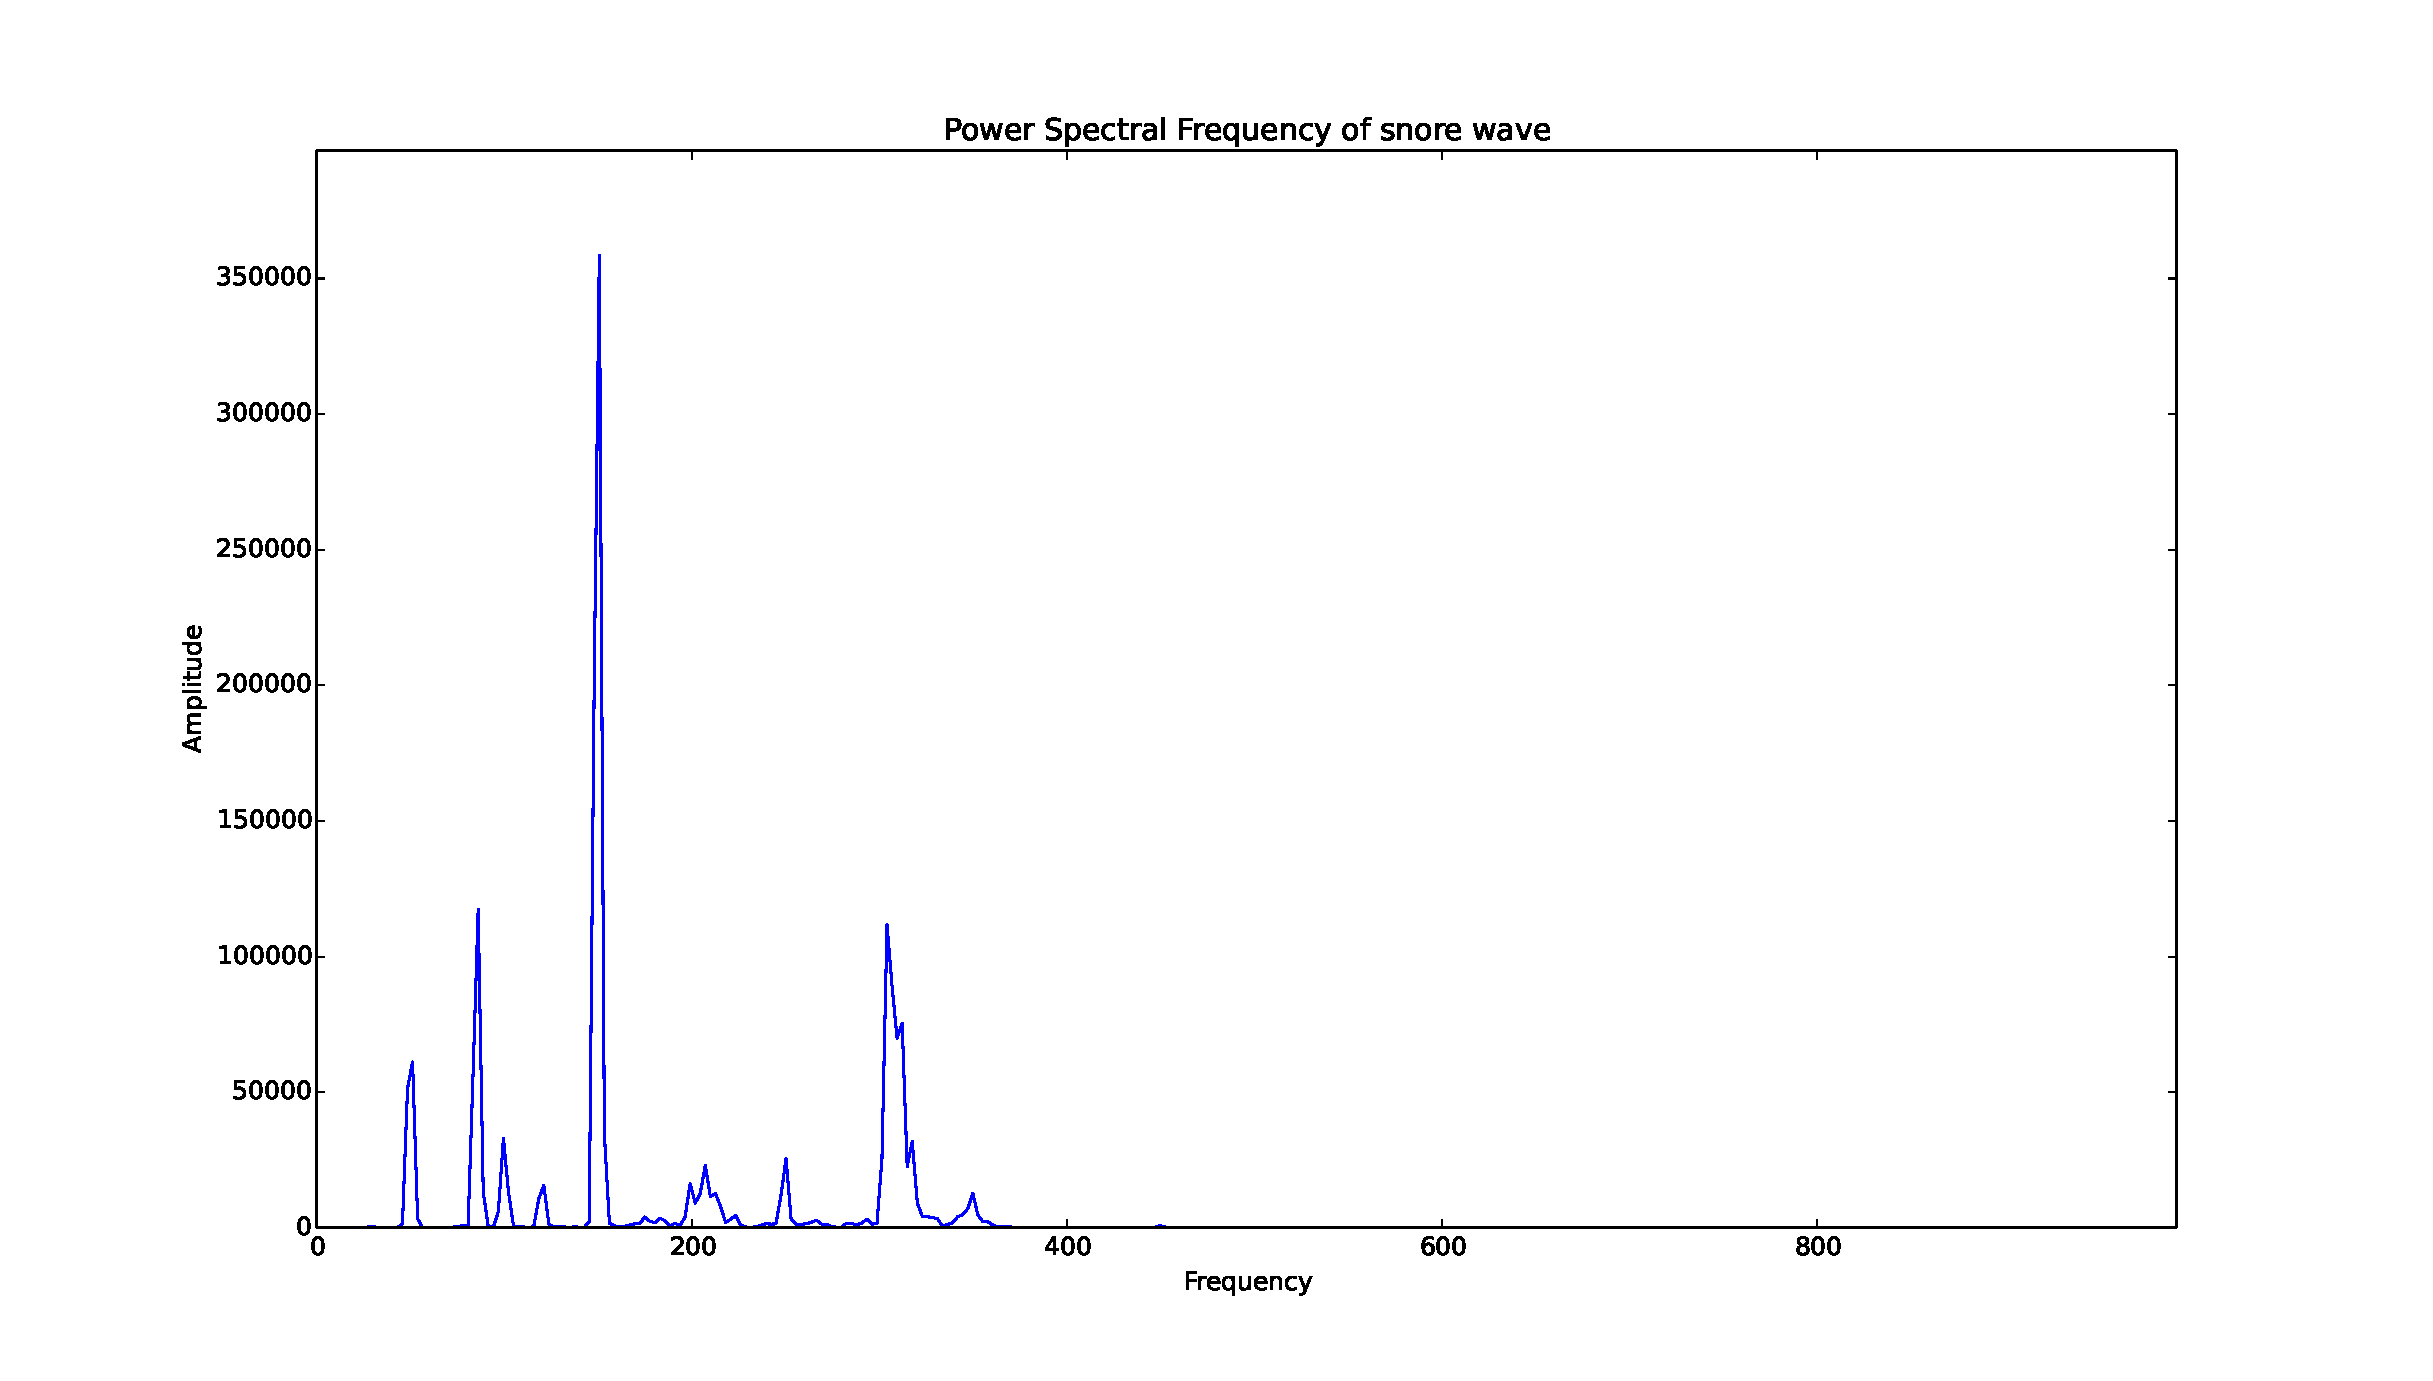
\includegraphics[width=15cm]{13_snorepsd.eps}
\caption{Power Spectral Density of the snore signal}
\label{fig:snorepsd}
\end{figure}

As it can be seen the snore signal has a set of specific properties in time domain, clearly observed by the spikes where the exhaling of air occurs. Even though time domain seems to be a good place to search for features, it actually contains too much of information and noise. That is the reason why signals are analyzed in frequency domain after prior preprocessing. Autocorrelation points out the relevant information in the signal and the frequency domain presents all the information in a concise manner.

The PSD is computed using Welch method via a wrapper around Matplotlib method available in \ref{list13}. The periodiogram is obtained by computing DFT. Then it is computed the squared magnitude of the signal. 


\lstinputlisting[language=Python, caption={PSD function}, label=list13]{../sourcecode/psd.py}

\subsubsection{Features and training}

Therefore the major task is to extract those peaks and their amplitude values. But the job of identified local maximas with no prior knowledge isn't trivial. At first it was attempted to detect the formants from the whole vector of data. In this case the formant was identified as such if it has a maximal value within a bin and is preceded to the left by a value lower than a specified $\delta$. The following method didn't work, because each vector was having a variable number of formants. There was no equivalent for the other signals to have or not have a feature at the same frequency as that signal had. Hence formants method was dropped, even though it identified correctly the formants, but couldn't guarantee to identify formants in the same frequency range for the other signals.

That's why it was chosen to detect local maxima from predefined ranges of the signal vector. Clearly this is peaking on the data and searching for the pattern using human input. For this specific snoring case the following ranges were detected: $(45, 55), (80, 90), (95, 105), (145, 155), (195, 205),$ $ (245, 255), (300, 310)$. The algorithm how checking the maxima in those areas is shown in \ref{list4}. The visualization of the peaks in \ref{fig:peaks} clearly shows how $7$ local maxima were identified, which makes it $14$ features, because both the frequency and the magnitude values are stored.

\begin{figure}[!ht]
\centering
  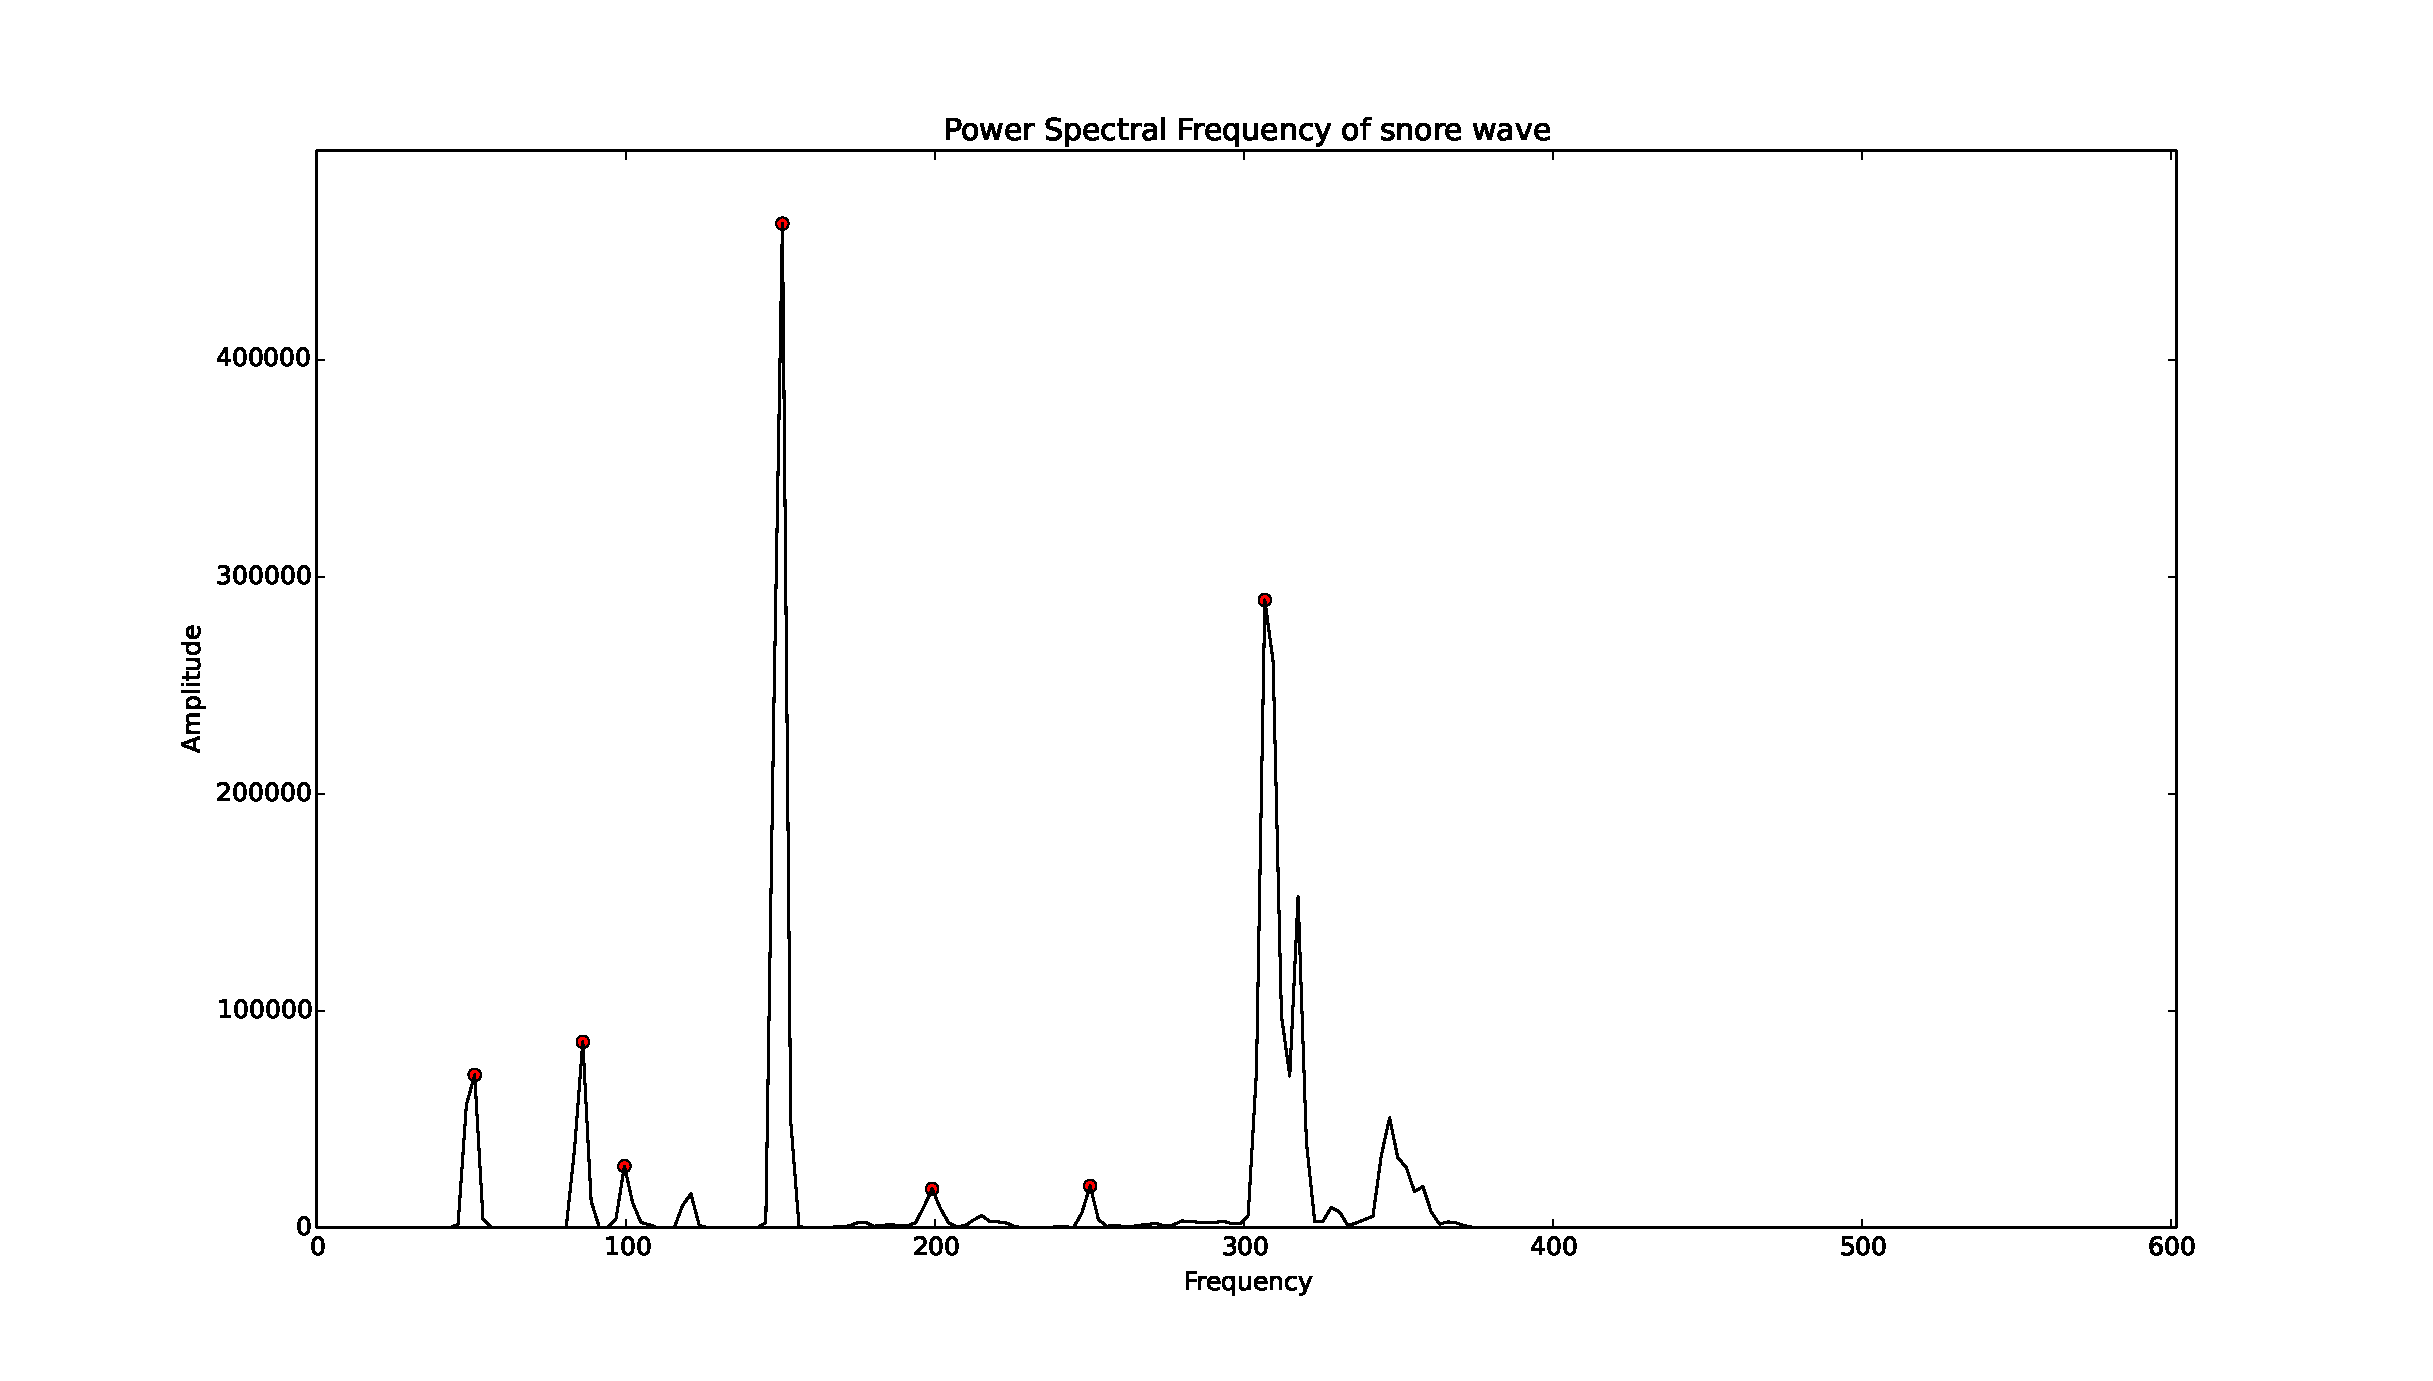
\includegraphics[width=15cm]{14_peaks.eps}
\caption{The peaks in PSD of a snore signal}
\label{fig:peaks}
\end{figure}

This is only one set of all the features. To ensure oneself that there are no other peaks or excess of data in the frequency domain, it was decided to compute also the areas of the bins. That includes splitting up the signal into bins of a specific window size and computing the area using composite trapezoidal rule presented in \ref{list5}. Only the first $20$ bins are taking into consideration, since only the low frequencies matter in this case. The window size was selected to be $40$ points. In total there are $34$ features for each sample. The number of features is much smaller than the number of samples, which is a good sign and hopefully all of the features are relevant to the regression algorithm.

In figure \ref{fig:peaks} the peaks are shown with red dots defined by specific frequencies and magnitudes. At first it might give the impression that the magnitude is not important. In fact it is, since the value of the magnitude determines a important property of the signal.

In figure \ref{fig:bins} an arbitrary number of bins is shown split by green vertical lines. Each bin contains a portion of the PSD. In that way it is possible to compute the area of each bin and keep all the values in the table of features.

\lstinputlisting[language=Python, caption={Extract bin areas function}, label=list5]{../sourcecode/bins.py}

\begin{figure}[!ht]
\centering
  \includegraphics[width=15cm]{18_psdbins.eps}
\caption{The visualization of bins in PSD}
\label{fig:bins}
\end{figure}

Before proceeding to training phase, the central question is where from to get the training data. For this project the data was kindly offered by Prague Psychiatric Center \cite{pcp} and it includes a $9$ hour recording of sleep sounds from a person diagnosed with Sleep Apnea. The snoring part estimates roughly to $6$ hours. The initial data was sampled at $44100$ Hz and resampled because of compression reasons to $11025$ Hz. The bottleneck here is the lack of snoring of a healthy person. In that way it would be possible to compare those two and identify the differences. 

Besides the positive examples fed to the classification algorithm, it is essential to acquire negative samples. Normally negative samples would include everything else. But it is hard to extract features from an infinite set of data. Therefore the infinity is shrinked to a set of most common noises during the night, like coughing, background noise from the streets, far airplane noises, sneezing, room silence. The negative samples were found from a free library of sounds \cite{freesounds}.

So by picking up positive and negative samples in total $5000$ samples each having $34$ features, the Logistic Regression model is build. The modeling is done using Sklean library that contains an interface to use Logistic Regression, therefore the code is pretty straight-forward shown in \ref{list6}. The coefficients of the training are stored in a JSON file for further predicting.

\lstinputlisting[language=Python, caption={Training using Logistic Regression}, label=list6]{../sourcecode/training.py}

\subsubsection{End user application}
This was the processing and training part described. Next is the end-user application build using Kivy framework, \cite{kivy}. Kivy is free and open source software. It runs on Android, iOS, Linux, OS X, and Windows. It is developed by the community along with the projects such as Python for Android, Kivy iOS. Kivy supports mouse, keyboard and multitouch platform specific events, contains a graphic library using OpenGL ES 2, has a range of Widgets. Kivy started as an initiative several years ago and becomes more and more popular among Python developers.

A simple application using Kivy was created to demonstrate how the detection works. The application was planned to be deployed mainly on Android platform, but unfortunately an important issue came out -- Kivy isn't yet having a stable module for signal input. The recommended way is using a recipe created by Kivy developers called ``audiostream'' library that deals with speakers and microphone on Android and iOS devices. Sadly the recipe is not guaranteed to work on any device and fails to capture the input from the microphone on popular Android phones.

\begin{figure}[!ht]
  \centering
  \subfloat[Sleep screen of the application\label{fig:screen1}]{%    
    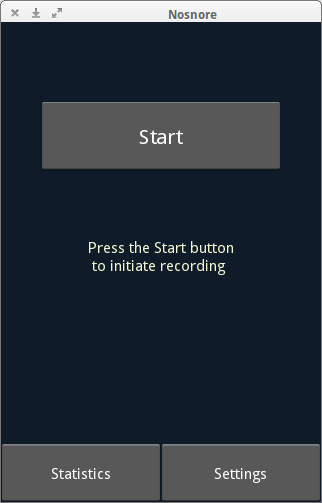
\includegraphics[width=0.4\textwidth]{screen1.png}      
  }
  \vspace{0.08cm}
  \subfloat[Settings screen of the application\label{fig:screen2}]{%
    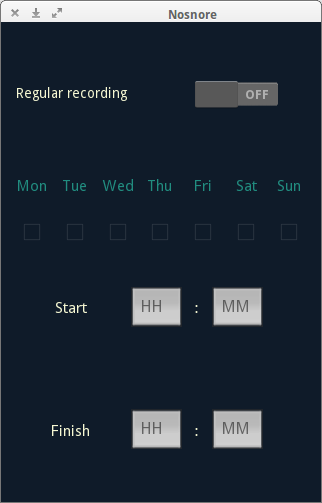
\includegraphics[width=0.4\textwidth]{screen2.png}
  }
  \caption{Application interface}
  \label{fig:screens}
\end{figure}

The recorder module presented in \ref{list8} shows several classes that perform the audio recording. The main class ``Recorder'' serves as a dispatcher and contains no real functionality. It determines the platform on which the application is running at the moment and decide which real recorder class should be used. Since there have been some issues with ``audiostream'' packages for audio input/output on mobile platforms, an example was provided for desktop environments. For recording audio on GNU/Linux, Mac and Windows systems the PyAudio version $0.2.8$ ([\cite{pyaudio}]) package has been used.

The audio recording is done with a sampling rate of $11024$ Hz, with a $1024$ framerate in mono mode, hence on a single channel. The recording is stored to a WAV file on the system with the time of recording encoded in its filename. The stream recording is started using PyAudion and the captured frames are written to the WAV file via a callback function.

The recording is toggled by the button. Here is an example of interaction of the screen object with the helper classes. It initializes the recorder object and binds the button to a callback method. When the button is triggered, the recording start or stops depending on the condition.

\lstinputlisting[language=Python, caption={SleepScreen class from kivy application}, label=list10]{../sourcecode/sleep_screen.py}

Hence the prototype works on desktop systems. The recommended way to use the application is to deploy it on a Raspberry Pi single-board computer and connect a USB microphone. The application has a simple interface and includes 3 screens. The sleep screen from figure \ref{fig:screen1} displays a single button to start and than stop the recording. The settings are set on figure \ref{fig:screen2} and it has the ability to set regular recording time.

The interface is using universal widgets and it's demanding any platform specific gestures -- everything can be done on any platform. The UI is written in kv language -- a special subset of Kivy for GUI building. A portion of the kv file is presented in \ref{list7}.

The recording made from start to the end is processed using the same DSP methods. After extracting the features from the signal portions those are classified using the predictions made by the model. The total time is computed and the time of snoring. This information is displayed right after the user clicks the stop button. As a conclusion this is the simple prototype build to demonstrate the functionality of the system.

In order to deploy the application on Android platform, even though it was an attempt with fruitless results, but might become relevant in the future, buildozer (\cite{buildozer}) was used. Buildozer offers automatic builds, automatic distribution, build validation. It is a generic Python package for Android / iOS and desktop. Currently the tool is in alpha phase. Buildozer provides a specification file, which is configured by the developer. The specification file includes settings such as title, icon, splash icon, target platform, included modules. 

\subsection{Testing and results}

In order to validate the results obtained by the trained model, it is essential to test the results. Testing is relevant for any type of application, nonetheless in machine learning it's impossible to create a model and not provide testing results. Therefore testing of ``snore'' vs ``nosnore'' regression was conducted.

As a rule of thumb in machine learning the acquired data should be split into 2 groups -- training and testing. Therefore $70\%$ of the data was used for training and $30\%$ for testing, i.e $3712$ samples for testing. The script that does the testing is listed in \ref{list8}. 

The coefficients are extracted from JSON file and the model is reconstructed from the trained state. The interaction with serialized JSON objects is done using a custom class for JSON manipulation, serialization and deserialization. Data is extracted from the training database and sent for prediction. For that matter prediction probabilities are also computed.

The desealization of the logistic regression object isn't straight forward, since it is composite object with reference to other objects. The standard desealization module is not able to manage complex objects, since it requires depth search through all the object attributes. Since the logistic regression has only 2 attributes pointing to other objects, the states of those are stored in the same JSON as well.

The number of negative testing samples is a bit larger than the number of positive data. This is due to the fact that positive data is a really specific class of sounds and negative data can be represented by a big variety of nighttime sounds.

\lstinputlisting[language=Python, caption={Test training Python script}, label=list8]{../sourcecode/test_training.py}


The worker showed in \ref{list8}  yields the following results:

\begin{itemize}[topsep=5pt, partopsep=0pt,itemsep=3pt,parsep=1pt]
 \item $3499$ correctly labeled samples;
 \item $213$ incorrectly labeled samples;
 \item $94.2618534483\%$ accuracy. 
\end{itemize}

About $94\%$ of success in identifying snoring is a reasonable result. The percentage will probably drop for the training data out of a different set, which means a different input device. There haven't been done any real-world testing of the system in a home environment, therefore it is unknown how the system will behave by receiving input from a wide variety of microphones. That is one reason to make the application open for anybody who wants to use, test or improve the existing codebase. 

\clearpage